\section{Kvadratno programiranje, KKT uvjeti, dualnost i analiza osjetljivosti}

\subsection{Opis problema i provjera konveksnosti}

Zadan je optimizacijski problem kvadratnog programiranja (engl. \textit{Quadratic Programming} -- QP) s dvije projektne varijable $x = [x_1, x_2]^T \in \mathbb{R}^2$ i dva ograničenja nejednakosti:
\begin{equation}
\min_{x \in \mathbb{R}^2} \quad f(x) = x_1^2 + 2x_2^2 - 0.3 x_1 x_2 + 2x_1 - 3x_2
\label{eq:qp_primal}
\end{equation}
uz ograničenja:
\begin{align}
g_1(x) &= a_{11} x_1 + a_{12} x_2 + 10 \leq 0, \label{eq:qp_g1} \\
g_2(x) &= a_{21} x_1 + a_{22} x_2 - 3 \leq 0, \label{eq:qp_g2}
\end{align}
gdje su nominalne numeričke vrijednosti koeficijenata:
\begin{equation}
a_{11} = -1, \quad a_{12} = -1, \quad a_{21} = 1, \quad a_{22} = -1.
\end{equation}
Ograničenja u eksplicitnom obliku glase:
\begin{align}
g_1(x) &= -x_1 - x_2 + 10 \leq 0 \iff x_1 + x_2 \geq 10, \\
g_2(x) &= x_1 - x_2 - 3 \leq 0 \iff x_1 - x_2 \leq 3.
\end{align}

\subsubsection{Matrični kanonski zapis i dokaz stroge konveksnosti}

Funkcija cilja $f(x)$ može se prikazati u simetričnom matričnom obliku:
\begin{equation}
f(x) = \frac{1}{2} x^T Q x + c^T x,
\label{eq:qp_canonical}
\end{equation}
gdje su Hesseova matrica $Q = \nabla^2 f(x) \in \mathbb{R}^{2 \times 2}$ i vektor linearnog dijela $c \in \mathbb{R}^2$ definirani kao:
\begin{equation}
Q = \begin{bmatrix} 2 & -0.3 \\ -0.3 & 4 \end{bmatrix}, \quad c = \begin{bmatrix} 2 \\ -3 \end{bmatrix}.
\end{equation}
Uvrštavanjem se potvrđuje identitet:
\begin{equation}
\frac{1}{2} \begin{bmatrix} x_1 & x_2 \end{bmatrix} \begin{bmatrix} 2 & -0.3 \\ -0.3 & 4 \end{bmatrix} \begin{bmatrix} x_1 \\ x_2 \end{bmatrix} + \begin{bmatrix} 2 & -3 \end{bmatrix} \begin{bmatrix} x_1 \\ x_2 \end{bmatrix} = x_1^2 + 2x_2^2 - 0.3 x_1 x_2 + 2x_1 - 3x_2 \equiv f(x).
\end{equation}

Da bi funkcija cilja $f(x)$ bila strogo konveksna na čitavom prostoru $\mathbb{R}^2$, nužno je i dovoljno da je Hesseova matrica $Q$ simetrična i strogo pozitivno definitna ($Q \succ 0$). Svojstvene vrijednosti matrice $Q$ određuju se iz karakterističnog polinoma:
\begin{equation}
\det(\lambda I - Q) = \det \begin{bmatrix} \lambda - 2 & 0.3 \\ 0.3 & \lambda - 4 \end{bmatrix} = (\lambda - 2)(\lambda - 4) - 0.09 = \lambda^2 - 6\lambda + 7.91 = 0.
\end{equation}
Rješenja karakteristične jednadžbe iznose:
\begin{equation}
\lambda_{1,2} = \frac{6 \pm \sqrt{36 - 4 \cdot 7.91}}{2} = \frac{6 \pm \sqrt{4.36}}{2} \approx \frac{6 \pm 2.088061}{2},
\end{equation}
odnosno:
\begin{equation}
\lambda_1 \approx 1.955969 > 0, \quad \lambda_2 \approx 4.044031 > 0.
\end{equation}
Budući da su obje svojstvene vrijednosti strogo pozitivne ($\lambda_i > 0$), matrica $Q$ je pozitivno definitna ($Q \succ 0$), što dokazuje da je funkcija cilja $f(x)$ **strogo konveksna**~\cite{boyd2004convex}.

\subsubsection{Konveksnost dopustivog skupa i globalna optimalnost}

Dopustivi skup $\mathcal{F} \subset \mathbb{R}^2$ definiran je presjekom dva poluprostora:
\begin{equation}
\mathcal{F} = \{x \in \mathbb{R}^2 \mid g_1(x) \leq 0, \; g_2(x) \leq 0\} = \{x \in \mathbb{R}^2 \mid A x \leq b\},
\end{equation}
gdje su:
\begin{equation}
A = \begin{bmatrix} -1 & -1 \\ 1 & -1 \end{bmatrix}, \quad b = \begin{bmatrix} -10 \\ 3 \end{bmatrix}.
\end{equation}
Budući da su funkcije ograničenja $g_1(x)$ i $g_2(x)$ afine (linearne), njihovi podnivo-skupovi su zatvoreni poluprostori, a presjek proizvoljnog broja konveksnih skupova je konveksan skup. Stoga je dopustivo područje $\mathcal{F}$ konveksan poliedar. 

Budući da je funkcija cilja $f(x)$ strogo konveksna, a dopustivi skup $\mathcal{F}$ neprazan i konveksan, razmatrani problem je **konveksan optimizacijski problem**, što jamči postojanje **jedinstvenog globalnog minimuma** $x^*$ koji ujedno zadovoljava Karush-Kuhn-Tuckerove (KKT) uvjete optimalnosti.

\subsection{Lagrangeova funkcija i KKT uvjeti optimalnosti}

Za problem~\eqref{eq:qp_primal}--\eqref{eq:qp_g2} definiramo Lagrangeovu funkciju $\mathcal{L}: \mathbb{R}^2 \times \mathbb{R}^2 \to \mathbb{R}$:
\begin{equation}
\mathcal{L}(x, \mu) = f(x) + \mu_1 g_1(x) + \mu_2 g_2(x) = f(x) + \mu^T (A x - b),
\end{equation}
gdje su $\mu = [\mu_1, \mu_2]^T$ Lagrangeovi množitelji pridruženi nejednakostima.

Gradijenti funkcije cilja i funkcija ograničenja iznose:
\begin{equation}
\nabla f(x) = Q x + c = \begin{bmatrix} 2x_1 - 0.3x_2 + 2 \\ 4x_2 - 0.3x_1 - 3 \end{bmatrix}, \quad \nabla g_1(x) = \begin{bmatrix} -1 \\ -1 \end{bmatrix}, \quad \nabla g_2(x) = \begin{bmatrix} 1 \\ -1 \end{bmatrix}.
\end{equation}

Karush-Kuhn-Tuckerovi (KKT) uvjeti prvog reda za konveksan QP predstavljaju nužne i dovoljne uvjete globalne optimalnosti~\cite{boyd2004convex,nocedal2006numerical}:
\begin{enumerate}
    \item \textbf{Stacionarnost Lagrangeove funkcije}:
    \begin{equation}
    \nabla_x \mathcal{L}(x^*, \mu^*) = \nabla f(x^*) + \mu_1^* \nabla g_1(x^*) + \mu_2^* \nabla g_2(x^*) = \begin{bmatrix} 0 \\ 0 \end{bmatrix},
    \label{eq:kkt_stat}
    \end{equation}
    odnosno:
    \begin{equation}
    \begin{bmatrix} 2 & -0.3 \\ -0.3 & 4 \end{bmatrix} \begin{bmatrix} x_1^* \\ x_2^* \end{bmatrix} + \begin{bmatrix} 2 \\ -3 \end{bmatrix} + \mu_1^* \begin{bmatrix} -1 \\ -1 \end{bmatrix} + \mu_2^* \begin{bmatrix} 1 \\ -1 \end{bmatrix} = \begin{bmatrix} 0 \\ 0 \end{bmatrix}.
    \end{equation}
    \item \textbf{Primarna dopustivost}:
    \begin{equation}
    g_1(x^*) = -x_1^* - x_2^* + 10 \leq 0, \quad g_2(x^*) = x_1^* - x_2^* - 3 \leq 0.
    \label{eq:kkt_primal}
    \end{equation}
    \item \textbf{Dualna dopustivost}:
    \begin{equation}
    \mu_1^* \geq 0, \quad \mu_2^* \geq 0.
    \label{eq:kkt_dual}
    \end{equation}
    \item \textbf{Komplementarno popuštanje}:
    \begin{equation}
    \mu_1^* \cdot (-x_1^* - x_2^* + 10) = 0, \quad \mu_2^* \cdot (x_1^* - x_2^* - 3) = 0.
    \label{eq:kkt_compl}
    \end{equation}
\end{enumerate}

\subsection{Analitičko rješavanje KKT sustava (4 kombinacije aktivnih skupova)}

Budući da imamo dva ograničenja nejednakosti, provodimo iscrpnu analizu svih $2^2 = 4$ mogućih kombinacija aktivnih i neaktivnih ograničenja.

\subsubsection{Slučaj 1: Oba ograničenja neaktivna ($\mu_1 = 0, \mu_2 = 0$)}

Ako nijedno ograničenje nije aktivno na granici, traži se stacionarna točka nesputane funkcije cilja:
\begin{equation}
\nabla f(x_0) = 0 \iff Q x_0 = -c \implies x_0 = -Q^{-1} c.
\end{equation}
Inverz matrice $Q$ iznosi:
\begin{equation}
Q^{-1} = \frac{1}{\det(Q)} \begin{bmatrix} 4 & 0.3 \\ 0.3 & 2 \end{bmatrix} = \frac{1}{7.91} \begin{bmatrix} 4 & 0.3 \\ 0.3 & 2 \end{bmatrix} = \frac{100}{791} \begin{bmatrix} 4 & 0.3 \\ 0.3 & 2 \end{bmatrix}.
\end{equation}
Računamo komponente nesputanog minimuma $x_0$:
\begin{equation}
x_0 = -\frac{100}{791} \begin{bmatrix} 4 & 0.3 \\ 0.3 & 2 \end{bmatrix} \begin{bmatrix} 2 \\ -3 \end{bmatrix} = -\frac{100}{791} \begin{bmatrix} 8 - 0.9 \\ 0.6 - 6 \end{bmatrix} = \begin{bmatrix} -\frac{710}{791} \\ \frac{540}{791} \end{bmatrix} \approx \begin{bmatrix} -0.897598 \\ 0.682680 \end{bmatrix}.
\end{equation}
Uvrštavanjem točke $x_0$ u ograničenja provjeravamo primarnu dopustivost:
\begin{equation}
g_1(x_0) = -(-0.897598) - 0.682680 + 10 = 10.214918 > 0.
\end{equation}
Budući da je $g_1(x_0) > 0$, nesputani optimum narušava primarno ograničenje te se **Slučaj 1 odbacuje kao primarno nedopustiv**.

\subsubsection{Slučaj 2: Samo prvo ograničenje aktivno ($\mu_1 > 0, \mu_2 = 0$)}

U ovom slučaju vrijedi $g_1(x) = 0 \implies x_1 + x_2 = 10$, dok je $\mu_2 = 0$. Uvjet stacionarnosti~\eqref{eq:kkt_stat} svodi se na sustav tri linearne jednadžbe s tri nepoznanice ($x_1, x_2, \mu_1$):
\begin{equation}
\begin{bmatrix} 2 & -0.3 & -1 \\ -0.3 & 4 & -1 \\ -1 & -1 & 0 \end{bmatrix} \begin{bmatrix} x_1 \\ x_2 \\ \mu_1 \end{bmatrix} = \begin{bmatrix} -2 \\ 3 \\ -10 \end{bmatrix}.
\end{equation}
Iz prve dvije jednadžbe izražavamo $\mu_1$:
\begin{align}
\mu_1 &= 2x_1 - 0.3x_2 + 2, \\
\mu_1 &= -0.3x_1 + 4x_2 - 3.
\end{align}
Izjednačavanjem desnih strana dobivamo:
\begin{equation}
2x_1 - 0.3x_2 + 2 = -0.3x_1 + 4x_2 - 3 \iff 2.3x_1 - 4.3x_2 + 5 = 0.
\end{equation}
Uvrštavanjem relacije $x_2 = 10 - x_1$ iz aktivnog ograničenja $g_1(x) = 0$:
\begin{equation}
2.3x_1 - 4.3(10 - x_1) + 5 = 0 \iff 6.6x_1 - 43 + 5 = 0 \iff 6.6x_1 = 38.
\end{equation}
Egzaktno analitičko rješenje glasi:
\begin{equation}
x_1^* = \frac{38}{6.6} = \frac{380}{66} = \frac{190}{33} \approx 5.757576,
\end{equation}
\begin{equation}
x_2^* = 10 - x_1^* = 10 - \frac{190}{33} = \frac{140}{33} \approx 4.242424.
\end{equation}
Lagrangeov množitelj $\mu_1^*$ iznosi:
\begin{equation}
\mu_1^* = 2\left(\frac{190}{33}\right) - 0.3\left(\frac{140}{33}\right) + 2 = \frac{380 - 42 + 66}{33} = \frac{404}{33} \approx 12.242424.
\end{equation}
Provjera svih KKT uvjeta za Slučaj 2:
\begin{enumerate}
    \item Dualna dopustivost: $\mu_1^* = \frac{404}{33} \approx 12.242424 > 0$ \quad \checkmark
    \item Primarna dopustivost za $g_2$:
    \begin{equation}
    g_2(x^*) = x_1^* - x_2^* - 3 = \frac{190}{33} - \frac{140}{33} - 3 = \frac{50}{33} - \frac{99}{33} = -\frac{49}{33} \approx -1.484848 < 0 \quad \checkmark
    \end{equation}
    \item Komplementarnost: $\mu_1^* g_1(x^*) = 0$ i $\mu_2^* g_2(x^*) = 0 \cdot (-1.4848) = 0$ \quad \checkmark
\end{enumerate}
Budući da su svi uvjeti zadovoljeni, točka $x^* = \left(\frac{190}{33}, \frac{140}{33}\right)$ s množiteljima $\mu^* = \left[\frac{404}{33}, 0\right]^T$ predstavlja **jedinstveni globalni optimum**.

Optimalna vrijednost funkcije cilja iznosi:
\begin{align}
p^* = f(x^*) &= \left(\frac{190}{33}\right)^2 + 2\left(\frac{140}{33}\right)^2 - 0.3\left(\frac{190}{33}\right)\left(\frac{140}{33}\right) + 2\left(\frac{190}{33}\right) - 3\left(\frac{140}{33}\right) \nonumber \\
&= \frac{2000}{33} \approx 60.606061.
\end{align}

\subsubsection{Slučaj 3: Samo drugo ograničenje aktivno ($\mu_1 = 0, \mu_2 > 0$)}

Postavljamo $g_2(x) = 0 \implies x_1 - x_2 = 3$ uz $\mu_1 = 0$. Sustav stacionarnosti daje:
\begin{equation}
\begin{bmatrix} 2 & -0.3 & 1 \\ -0.3 & 4 & -1 \\ 1 & -1 & 0 \end{bmatrix} \begin{bmatrix} x_1 \\ x_2 \\ \mu_2 \end{bmatrix} = \begin{bmatrix} -2 \\ 3 \\ 3 \end{bmatrix}.
\end{equation}
Rješavanjem ovog sustava dobivamo:
\begin{equation}
x_1 = \frac{121}{54} \approx 2.240741, \quad x_2 = -\frac{41}{54} \approx -0.759259, \quad \mu_2 = -\frac{3623}{540} \approx -6.709259.
\end{equation}
Provjera ograničenja $g_1(x)$:
\begin{equation}
g_1(x) = -2.240741 - (-0.759259) + 10 = 8.518519 > 0.
\end{equation}
Budući da je $\mu_2 < 0$ (kršenje dualne dopustivosti) i $g_1(x) > 0$ (kršenje primarne dopustivosti), \textbf{Slučaj 3 se odbacuje}.

\subsubsection{Slučaj 4: Oba ograničenja aktivna ($\mu_1 > 0, \mu_2 > 0$)}

Aktivnost oba ograničenja definira sjecište pravaca:
\begin{equation}
\begin{cases} -x_1 - x_2 = -10 \\ x_1 - x_2 = 3 \end{cases} \implies x_1 = 6.5, \quad x_2 = 3.5.
\end{equation}
Uvrštavanjem točke $x = [6.5, 3.5]^T$ u uvjet stacionarnosti $Q x + c + A^T \mu = 0$:
\begin{equation}
\begin{bmatrix} -1 & 1 \\ -1 & -1 \end{bmatrix} \begin{bmatrix} \mu_1 \\ \mu_2 \end{bmatrix} = -\begin{bmatrix} 2(6.5) - 0.3(3.5) + 2 \\ 4(3.5) - 0.3(6.5) - 3 \end{bmatrix} = -\begin{bmatrix} 13.95 \\ 9.05 \end{bmatrix}.
\end{equation}
Rješavanjem $2 \times 2$ sustava za množitelje:
\begin{equation}
\mu_1 = 11.50 > 0, \quad \mu_2 = -2.45 < 0.
\end{equation}
Budući da je $\mu_2 = -2.45 < 0$, narušen je uvjet dualne dopustivosti ($\mu_2 \geq 0$). Prema tome, \textbf{Slučaj 4 se odbacuje}.

\subsection{Geometrijska interpretacija i ravnoteža gradijenata}

Na slici~\ref{fig:qp_primal} prikazana je geometrija QP problema u ravnini $(x_1, x_2)$. Dopustivo područje $\mathcal{F}$ osjenčano je plavom bojom, eliptične nivo-krivulje prikazuju funkciju cilja $f(x)$, a zvjezdicom je označen optimalni vektor $x^*$.

\begin{figure}[H]
    \centering
    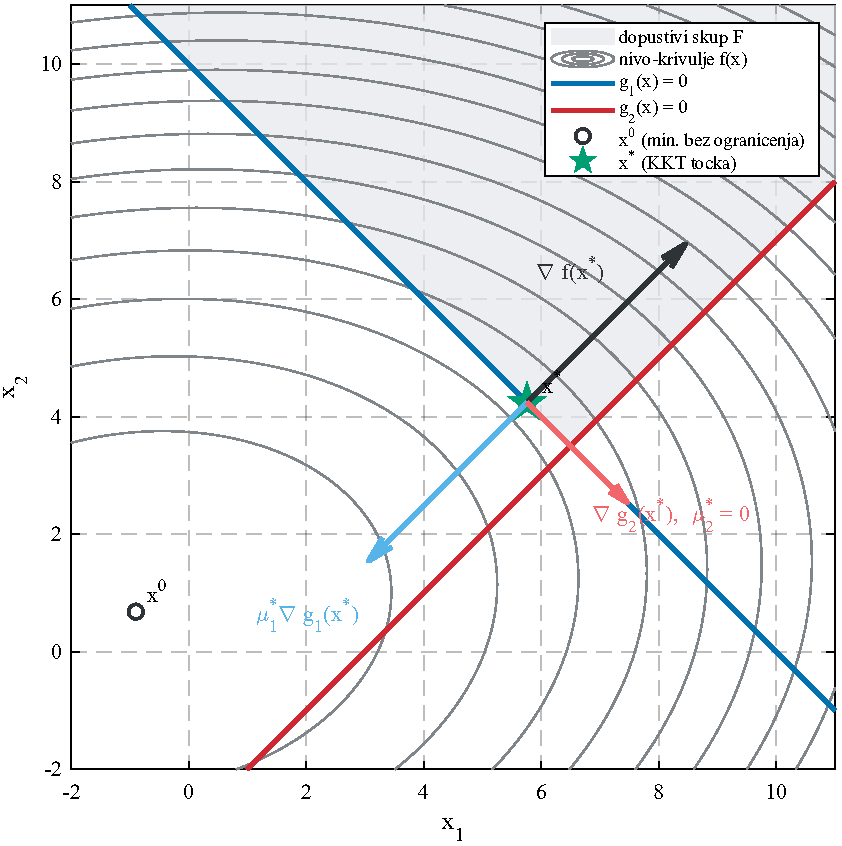
\includegraphics[width=0.82\textwidth]{figures/fig1_1_qp_primal_geometry.pdf}
    \caption{Geometrijski prikaz dopustivog skupa $\mathcal{F}$, nivo-krivulja funkcije cilja $f(x)$ i vektora gradijenata u KKT točki $x^*$.}
    \label{fig:qp_primal}
\end{figure}

U optimalnoj točki $x^* = (5.758, 4.242)$ gradijent funkcije cilja i gradijent aktivnog ograničenja iznose:
\begin{equation}
\nabla f(x^*) = \begin{bmatrix} 12.242424 \\ 12.242424 \end{bmatrix}, \quad \nabla g_1(x^*) = \begin{bmatrix} -1 \\ -1 \end{bmatrix}.
\end{equation}
Uočava se savršena kolinearnost suprotnog smjera:
\begin{equation}
\nabla f(x^*) + \mu_1^* \nabla g_1(x^*) = \begin{bmatrix} 12.242424 \\ 12.242424 \end{bmatrix} + 12.242424 \begin{bmatrix} -1 \\ -1 \end{bmatrix} = \begin{bmatrix} 0 \\ 0 \end{bmatrix}.
\end{equation}
Fizička interpretacija ovog uvjeta odgovara ravnoteži sila: gradijent funkcije cilja $\nabla f(x^*)$ teži pomaknuti točku prema unutrašnjosti (nesputanom minimumu $x_0$), no nailazi na reakciju veze (graničnu silu) normalnog vektora $\nabla g_1(x^*)$ proporcionalnu intenzitetu Lagrangeovog množitelja $\mu_1^* = 12.2424$.

\subsection{Numerička verifikacija u programskim paketima}

Problem je numerički verificiran u programskim alatima MATLAB (\texttt{quadprog}, YALMIP) i Python (\texttt{scipy.optimize}, \texttt{cvxpy}). U tablici~\ref{tab:qp_comparison} prikazana je usporedba analitičkih i numeričkih rezultata.

\begin{table}[H]
\centering
\caption{Usporedba analitičkih i numeričkih rezultata za Zadatak 1.}
\label{tab:qp_comparison}
\begin{tabular}{lcccc}
\toprule
\textbf{Veličina} & \textbf{Analitička vrijednost} & \textbf{MATLAB / Python} & \textbf{Apsolutna pogreška} & \textbf{Status} \\
\midrule
$x_1^*$ & $190/33 \approx 5.757576$ & $5.757576$ & $< 10^{-8}$ & Egzaktno \\
$x_2^*$ & $140/33 \approx 4.242424$ & $4.242424$ & $< 10^{-8}$ & Egzaktno \\
$\mu_1^*$ & $404/33 \approx 12.242424$ & $12.242424$ & $< 10^{-8}$ & Egzaktno \\
$\mu_2^*$ & $0.000000$ & $0.000000$ & $0.00$ & Neaktivno \\
$p^* = f(x^*)$ & $2000/33 \approx 60.606061$ & $60.606061$ & $< 10^{-8}$ & Egzaktno \\
$d^* = g(\mu^*)$ & $2000/33 \approx 60.606061$ & $60.606061$ & $< 10^{-8}$ & Jaka dualnost \\
\bottomrule
\end{tabular}
\end{table}

\subsection{Lagrangeova dualnost i dokaz jake dualnosti}

Lagrangeova dualna funkcija $g(\mu)$ definirana je kao infimum Lagrangeove funkcije po $x \in \mathbb{R}^2$~\cite{boyd2004convex,jokic2024predavanja}:
\begin{equation}
g(\mu) = \inf_{x \in \mathbb{R}^2} \mathcal{L}(x, \mu) = \inf_{x \in \mathbb{R}^2} \left[ \frac{1}{2} x^T Q x + (c + A^T \mu)^T x - b^T \mu \right].
\end{equation}
Budući da je $Q \succ 0$, funkcija unutar infimuma je strogo konveksna po $x$, a minimum se postiže poništavanjem gradijenta $\nabla_x \mathcal{L} = Q x + c + A^T \mu = 0$:
\begin{equation}
x^*(\mu) = -Q^{-1} (c + A^T \mu).
\label{eq:x_mu_dual}
\end{equation}
Uvrštavanjem $x^*(\mu)$ natrag u Lagrangeovu funkciju dobiva se eksplicitni analitički oblik dualne funkcije:
\begin{align}
g(\mu) &= \frac{1}{2} (-Q^{-1}(c + A^T \mu))^T Q (-Q^{-1}(c + A^T \mu)) + (c + A^T \mu)^T (-Q^{-1}(c + A^T \mu)) - b^T \mu \nonumber \\
&= -\frac{1}{2} (c + A^T \mu)^T Q^{-1} (c + A^T \mu) - b^T \mu.
\label{eq:dual_fun_explicit}
\end{align}
Budući da je matrica $-Q^{-1}$ negativno definitna, dualna funkcija $g(\mu)$ je konkavna kvadratna funkcija po $\mu = [\mu_1, \mu_2]^T$.

Lagrangeov dualni problem glasi:
\begin{equation}
\max_{\mu \in \mathbb{R}^2} \quad g(\mu) \quad \text{uz} \quad \mu_1 \geq 0, \; \mu_2 \geq 0.
\label{eq:dual_problem}
\end{equation}

\begin{figure}[H]
    \centering
    \includegraphics[width=0.78\textwidth]{figures/fig1_2_qp_dual_surface.pdf}
    \caption{Nivo-krivulje konkavne Lagrangeove dualne funkcije $g(\mu_1, \mu_2)$ i optimalna dualna točka $\mu^* = (12.242, 0.000)$.}
    \label{fig:qp_dual}
\end{figure}

Slika~\ref{fig:qp_dual} prikazuje nivo-krivulje dualne funkcije $g(\mu_1, \mu_2)$. Numeričkim rješavanjem pomoću funkcije \texttt{fmincon} (minimizacija funkcije $-g(\mu)$ uz $\mu \geq 0$) dobiva se:
\begin{equation}
\mu^* = \begin{bmatrix} 12.242424 \\ 0.000000 \end{bmatrix}, \quad d^* = g(\mu^*) = 60.606061.
\end{equation}

\subsubsection{Provjera Slaterovog uvjeta i jaka dualnost}

Slaterov teorem o jakoj dualnosti jamči da za konveksan problem s afinim ograničenjima vrijedi nulti dualni procjep ($p^* = d^*$) ako postoji točka $x_{\mathrm{int}}$ u strogoj unutrašnjosti dopustivog skupa~\cite{boyd2004convex}. Odabirom točke $x_{\mathrm{int}} = [7, 6]^T$ imamo:
\begin{equation}
g_1(x_{\mathrm{int}}) = -7 - 6 + 10 = -3 < 0, \quad g_2(x_{\mathrm{int}}) = 7 - 6 - 3 = -2 < 0.
\end{equation}
Budući da je Slaterov uvjet strogo zadovoljen, vrijedi **jaka dualnost**:
\begin{equation}
\gamma = p^* - d^* = 60.606061 - 60.606061 = 0.
\end{equation}

\subsection{Analiza osjetljivosti i perturbacija ograničenja}

Teorem o osjetljivosti u nelinearnom programiranju povezuje optimalne Lagrangeove množitelje s parcijalnim derivacijama optimalne vrijednosti funkcije cilja po desnim stranama ograničenja~\cite{boyd2004convex,bertsekas2016nonlinear}. 

Neka je $p^*(u)$ funkcija optimalne vrijednosti u ovisnosti o perturbacijskom vektoru $u = [u_1, u_2]^T$, gdje su ograničenja perturbirana u obliku $A x \leq b + u$:
\begin{equation}
p^*(u) = \inf \{f(x) \mid A x \leq b + u\}.
\end{equation}
Prema teoremu o osjetljivosti vrijedi:
\begin{equation}
\frac{\partial p^*}{\partial b_i} = -\mu_i^*, \quad i = 1, 2.
\label{eq:sensitivity_thm}
\end{equation}
Za naša ograničenja dobivamo:
\begin{equation}
\frac{\partial p^*}{\partial b_1} = -\mu_1^* = -\frac{404}{33} \approx -12.242424, \quad \frac{\partial p^*}{\partial b_2} = -\mu_2^* = 0.
\end{equation}

\begin{figure}[H]
    \centering
    \includegraphics[width=0.78\textwidth]{figures/fig1_3_qp_sensitivity.pdf}
    \caption{Funkcija optimalne vrijednosti $p^*(b_1 + \Delta b_1)$ u usporedbi s linearnom aproksimacijom nagiba $-\mu_1^*$.}
    \label{fig:qp_sensitivity}
\end{figure}

\subsubsection{Inženjerska i ekonomska interpretacija (cijene u sjeni)}

Množitelj $\mu_1^* = 12.2424$ ima ulogu \textbf{cijene u sjeni} (\textit{shadow price}):
\begin{itemize}
    \item Ako se desna strana prvog ograničenja $b_1$ poveća za mali iznos $\Delta b_1 > 0$ (čime se ograničenje $-x_1 - x_2 \leq -10 + \Delta b_1$ relaksira), optimalna vrijednost $p^*$ se \textbf{smanjuje} po stopi od približno $12.2424 \cdot \Delta b_1$.
    \item Ako se desna strana drugog ograničenja $b_2$ perturbira, budući da je $g_2$ neaktivno ($\mu_2^* = 0$), to nema nikakvog utjecaja na optimalno rješenje prvog reda ($\frac{\partial p^*}{\partial b_2} = 0$).
\end{itemize}

Numerička verifikacija provedena je s perturbacijskim korakom $\Delta b_1 = 10^{-4}$:
\begin{equation}
\left( \frac{\Delta p^*}{\Delta b_1} \right)_{\mathrm{num}} = \frac{p^*(b_1 + 10^{-4}) - p^*(b_1)}{10^{-4}} = -12.242357,
\end{equation}
što daje odstupanje od analitičke derivacije manje od $6.75 \times 10^{-5}$, čime je teorem osjetljivosti u potpunosti verificiran.
